\documentclass[a4paper,12pt]{report}
\usepackage{graphicx}
\title{Tugas pemrograman 2}
\author{Nuha Hanifatul Khonsa'}
\date{17 oktober 2019}
\begin{document}


\maketitle

\chapter{}
\section{Sejarah Python}
\usepackage{Pencipta bahasa pemrograman Python adalah Guido van Rossum di Centrum Wiskunde dan Informatica (CWI) di Belanda pada awal tahun 1990an. Bahasa Python sendiri terinspirasi dari bahasa pemrograman ABC.Bahasa Python sendiri bersifat open source sehingga dapat memungkinkan ribuan orang untuk dapat berkonstribusi dalam mengembangkannya.
Pada tahun 1995, Guido melanjutkan pembuatan Python di Corporation for National Research Initiative (CNRC) di Virginia Amerika. Lalu pada tahun 2000, Guido dan tim Python pindah ke BeOpen.com dan membentuk PythonLabs hingga pada tahun 2001 terbentuklah organisasi Python ialah Python Software Foundation(PSF.)
Python tersedia untuk berbagai macam system operasi seperti Unix(linux), PCs (DOS, Windows, OS/2) dan lainnya.
}

\section{Perbedaan Python 2 dan Python 3}
\usepackage{Ada 2 versi Python yang sering digunakan  saat ini pada lingkungan pengembangan dan produksi  yaitu Python 2 dan Python 3}
\paragraph{Perbedaan diantara keduanya ialah Python 2 sendiri merupakan versi dari bahasa pemrograman python yang banyak digunakan sementara Python 3 adalah pengembangan dari Python 2 yang memiliki fitur lebih. Sedangkan perintah yang digunakan Python 2 menggunakan perintah python saja, sedangkan Python 3 menggunakan perintah  python3}

\section{Implementasi dan penggunaan Python pada Perusahaan}
\usepackage{Pengggunaan Python sebagai Data Science dan Data Mechine Learning sangat berpengaruh dalam perkembangan tiap lini yang ada baik pada kesehatan, pendidikan bahkan pada kebutuhan sebuah perusahaan terutama bidang IT.}
\textbf{Perusahaan yang menggunakan Python antara lain :}
\begin{enumerate}
    \item Google : menggunakan Python pada mesin pencarian
    \item Youtube : sebagai situs video terbesar dan terpopuler di dunia, sebagian besar kode dalam Youtube ditulis dalam bahasa Python.
    \item Facebook : media sosial terbesar di dunia bahkan sebagai media social yang tidak memandang tingkatan ini menggunakan Tornado sebuah framework Python untuk menampilkan timeline.
    \item Instagram : Instagram menggunakan Django, framework python sebagai mesin pengolah sisi server dari aplikasinya.

\end{enumerate}
   
\chapter{Instalasi}
\section{Instalasi Anaconda}
\usepackage{Berikut Langkah dalam Menginslas Anaconda:}
\begin{enumerate}
    \item Sebagai langkah awal dan langkah penting dalam instalasi anaconda adalah kita harus memiliki Installer Anaconda itu sendiri.
    \item Jika belum memilikinya kita dapat mendownload instaleller anaconda terlebih dahulu atau jika tidak mau mendownload sendiri kita dapat meminta installer kepada teman yang punya.
    \item Langkah selanjutnya buka file installer lalu klik 2x  
    \item Pada tahap instalasi pertama ini kita pilih Next
    \item Lalu akan muncul License Agreement pilih I Agree
    \item Kemudian pada Select Instalation Type ada 2 pilihan yaitu Just Me pilihan ini dimana hanya pada 1 user dan user lain di laptop tidak bisa menggunakannya dan pilihan  All User pilihan dimana semua user dapat menggunakannya, 
    \item Selanjutnya pilih lokasi penyimpanan. Lokasi penyimpanan sesuai keinginan kita lalu klik Next
    \item Pada bagian Add Environment ceklis ke 2 nya dan Klik Install
    \item Lalu tunggu instalasi sampai selesai
    \item Kemudian akan muncul Instalation Complate lalu klik Next.
    \item Lalu klik FINISH
    \item Kita dapat membuka hasil instalasi pada Anaconda Navigator
\end{enumerate}

\section{Cek instalasi Pip}
\usepackage{Untuk menecek apakah ‘pip’ telah terinstal pada laptop kita dengan cara membuka Command Prompt lalu ketik kan ”pip –version”.}

\section{Setting Environment}
\usepackage{Berikut Langkah-Langkah setting Environment:}
\begin{enumerate}
    \item Buka Control Panel
    \begin{center}
        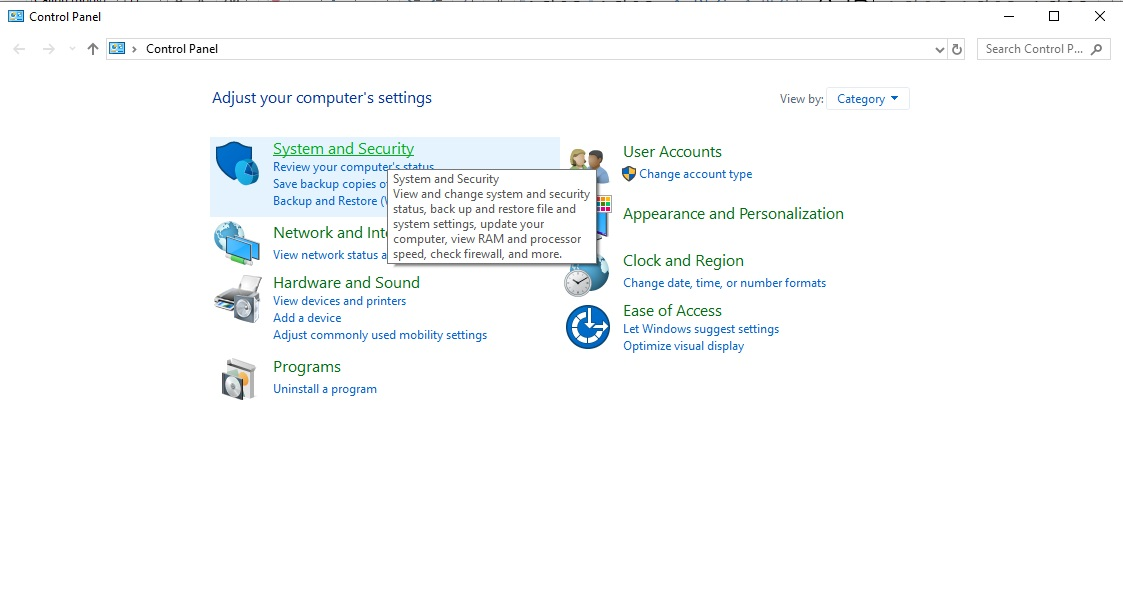
\includegraphics[width=10cm\textwidth]{environment1.jpg}
    \end{center}
    \item Lalu pilih System and Security
    \begin{center}
          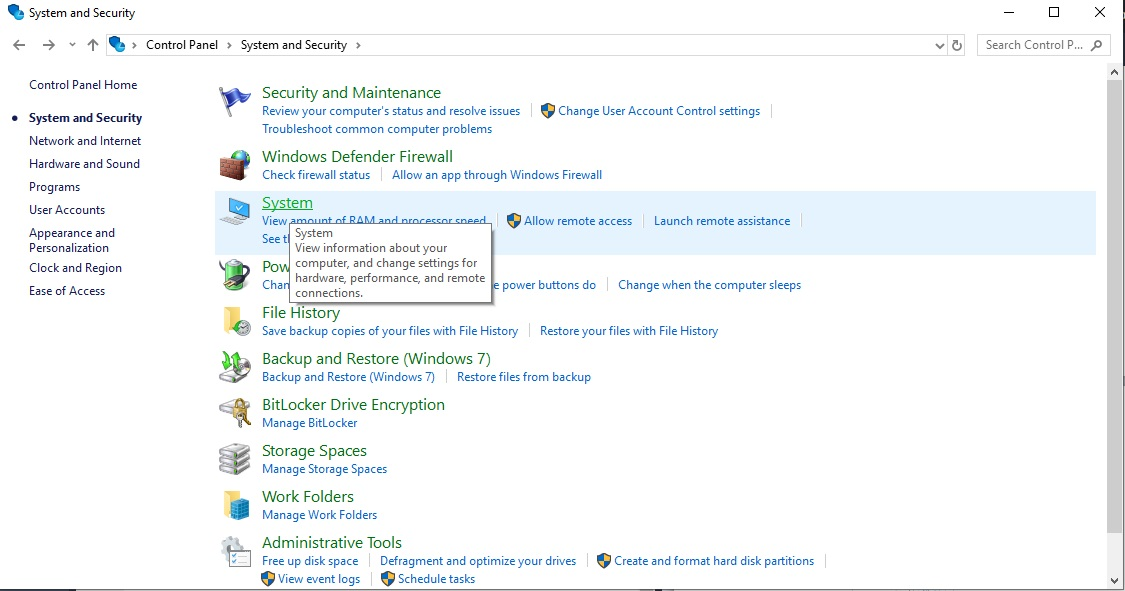
\includegraphics[width=8cm\textwidth]{system.jpg}
    \end{center}
    \item Selanjutnya pilih System
    \begin{center}
          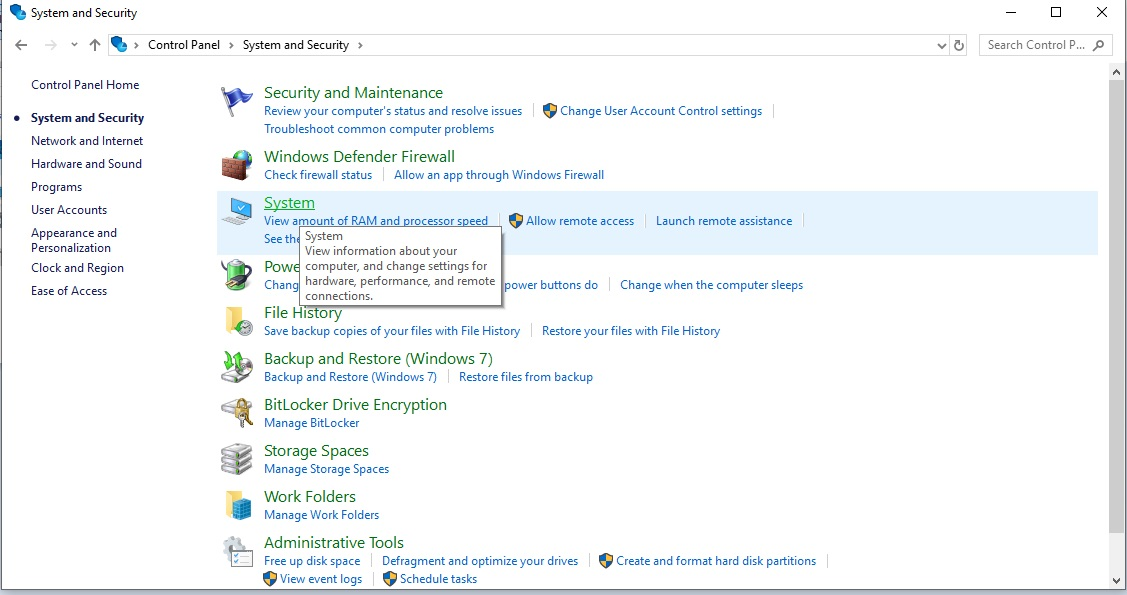
\includegraphics[width=8cm\textwidth]{environment2.jpg}
    \end{center}
    \item Kemudian pilih Advanced system settings pada sisi kiri
    \begin{center}
          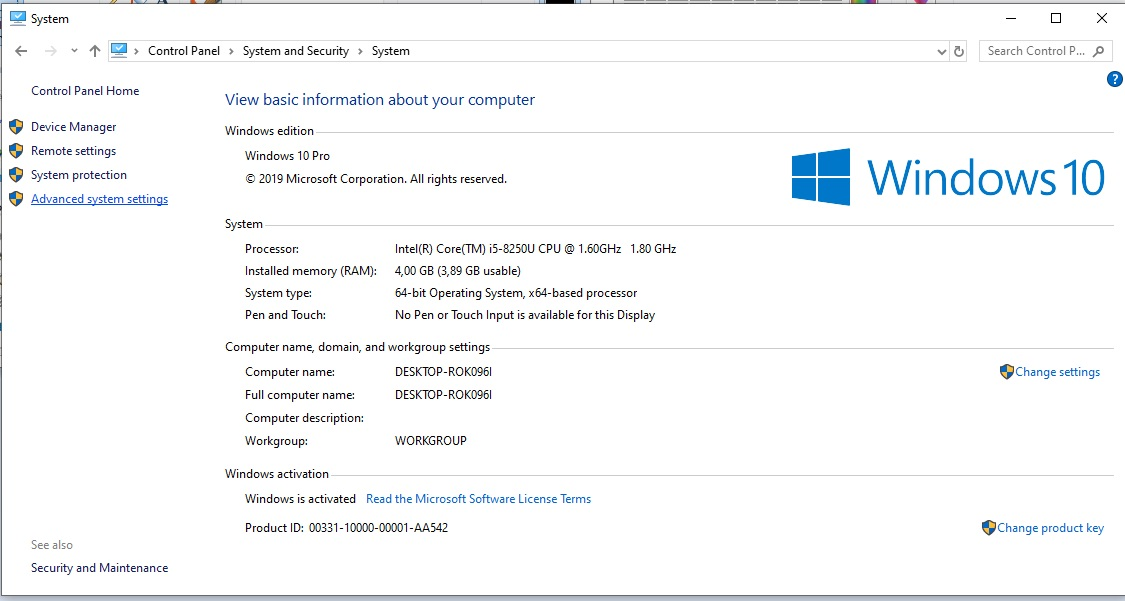
\includegraphics[width=8cm\textwidth]{environment3.jpg}
    \end{center}
    \item Pada System Properties pilih Environment Variable
    \begin{center}
          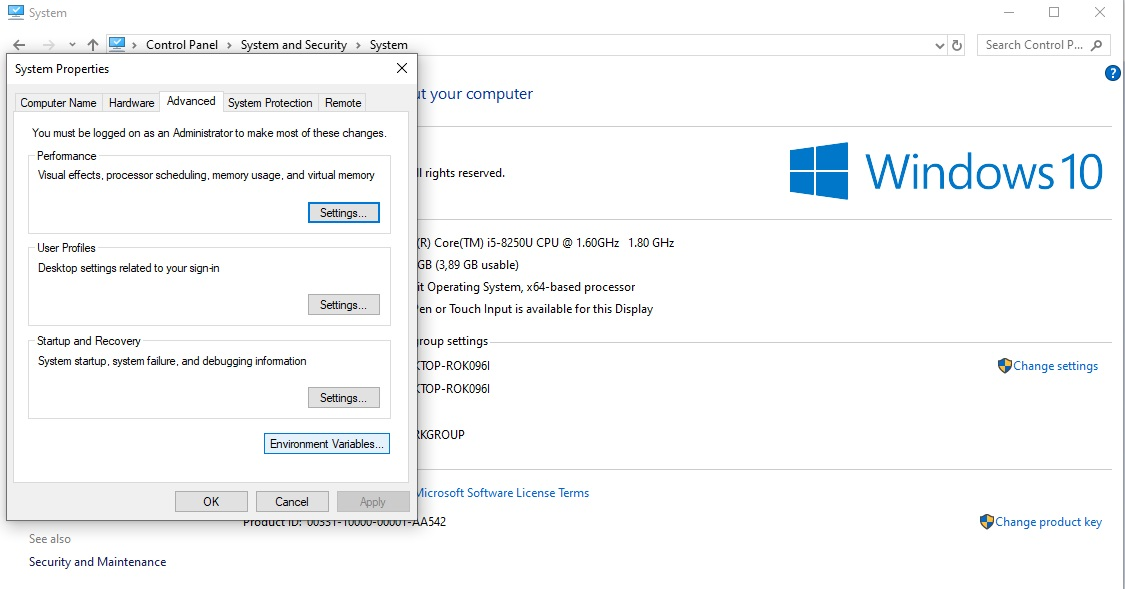
\includegraphics[width=8cm\textwidth]{environment4.jpg}
    \end{center}
    \item Lalu klik Oke pada  Environment Variable
    \begin{center}
        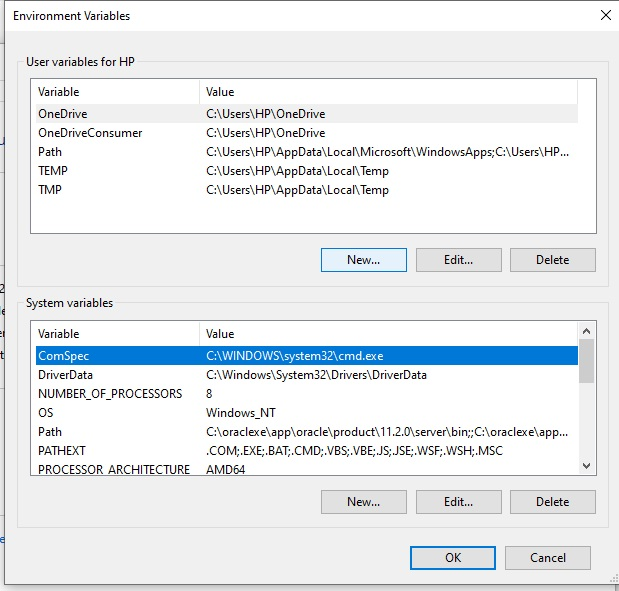
\includegraphics[width=8cm\textwidth]{environment5.jpg}
    \end{center}
\end{enumerate}

\chapter{}
\section{Penggunaan Spyder}
\begin{enumerate}
    \item Membuat file baru
    \begin{center}
        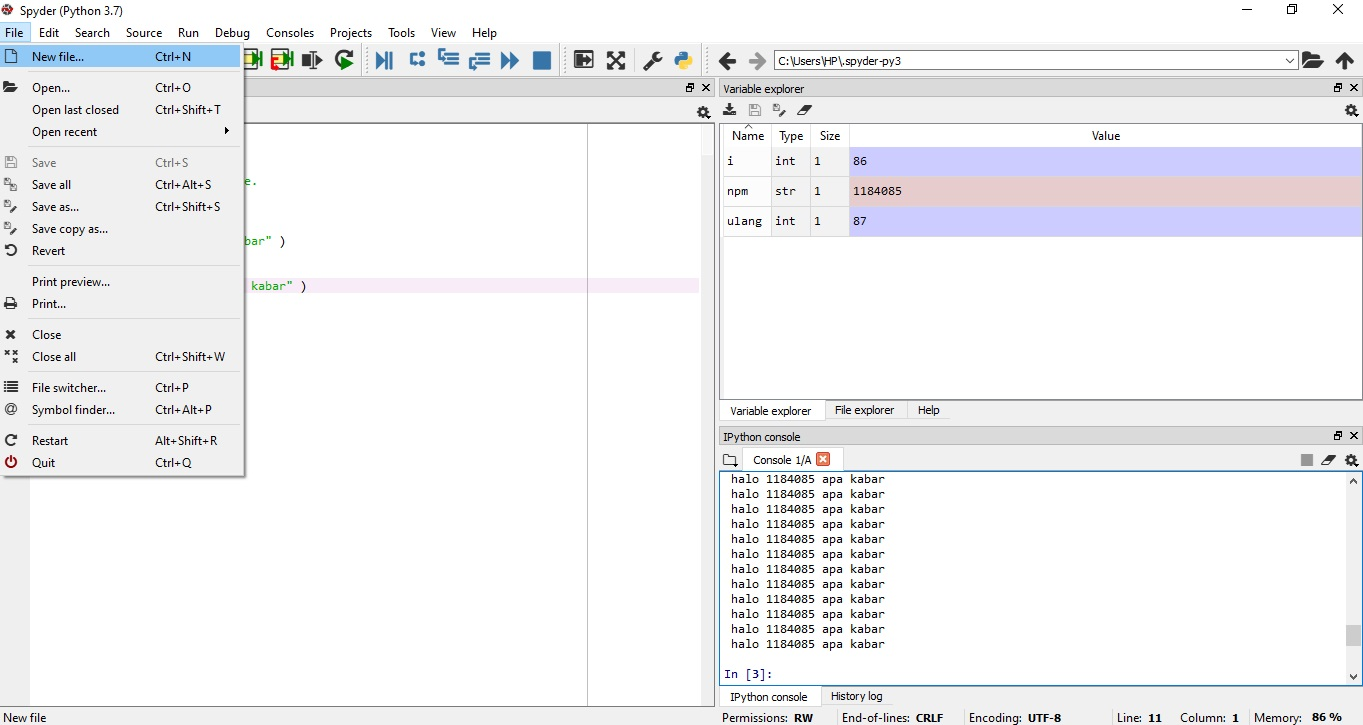
\includegraphics[width=8cm\textwidth]{spyder1.jpg}
    \end{center}
    \item Tuliskan ' print("Hello World")'
    \begin{center}
        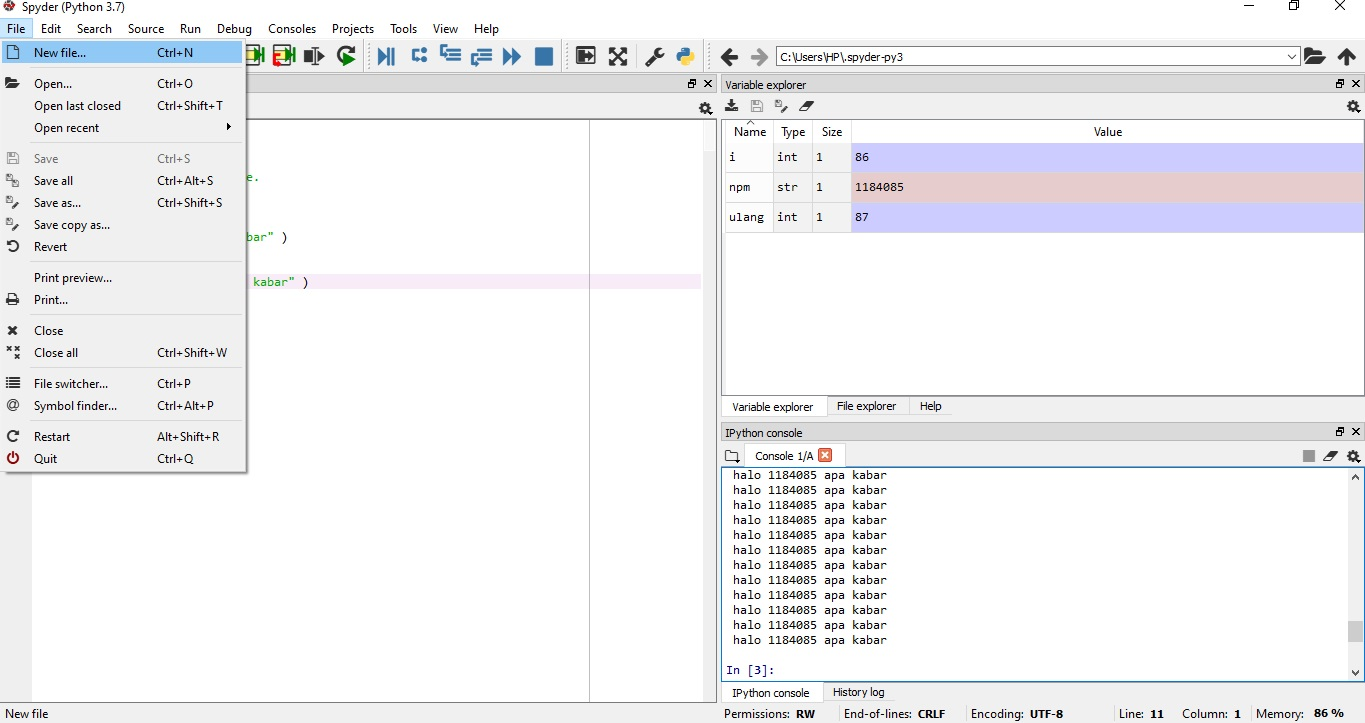
\includegraphics[width=8cm\textwidth]{spyder2.jpg}
    \end{center}
    \item Klik Run pada icon sseperti icon play berwarna hijau
    \item Lalu save file
    \begin{center}
        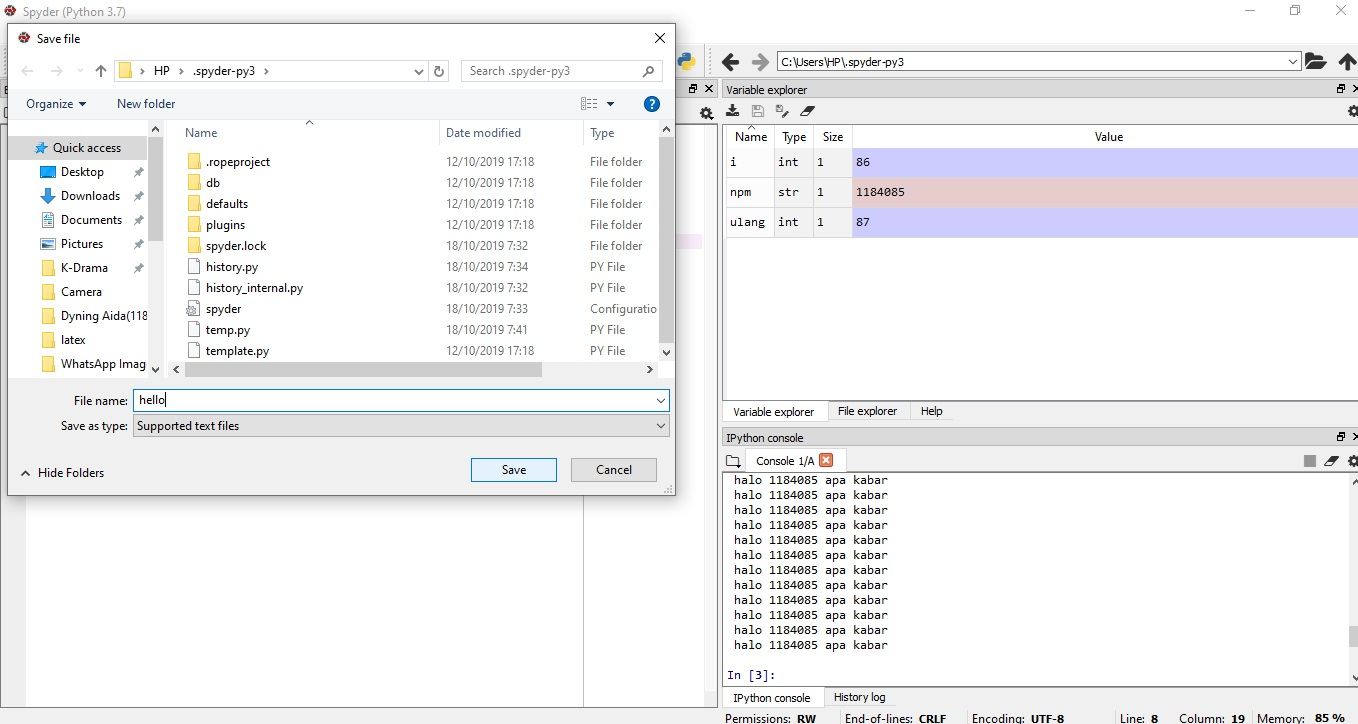
\includegraphics[width=8cm\textwidth]{spyder3.jpg}
    \end{center}
    \item Print Hello World pada consule di kanan bawah
    \begin{center}
        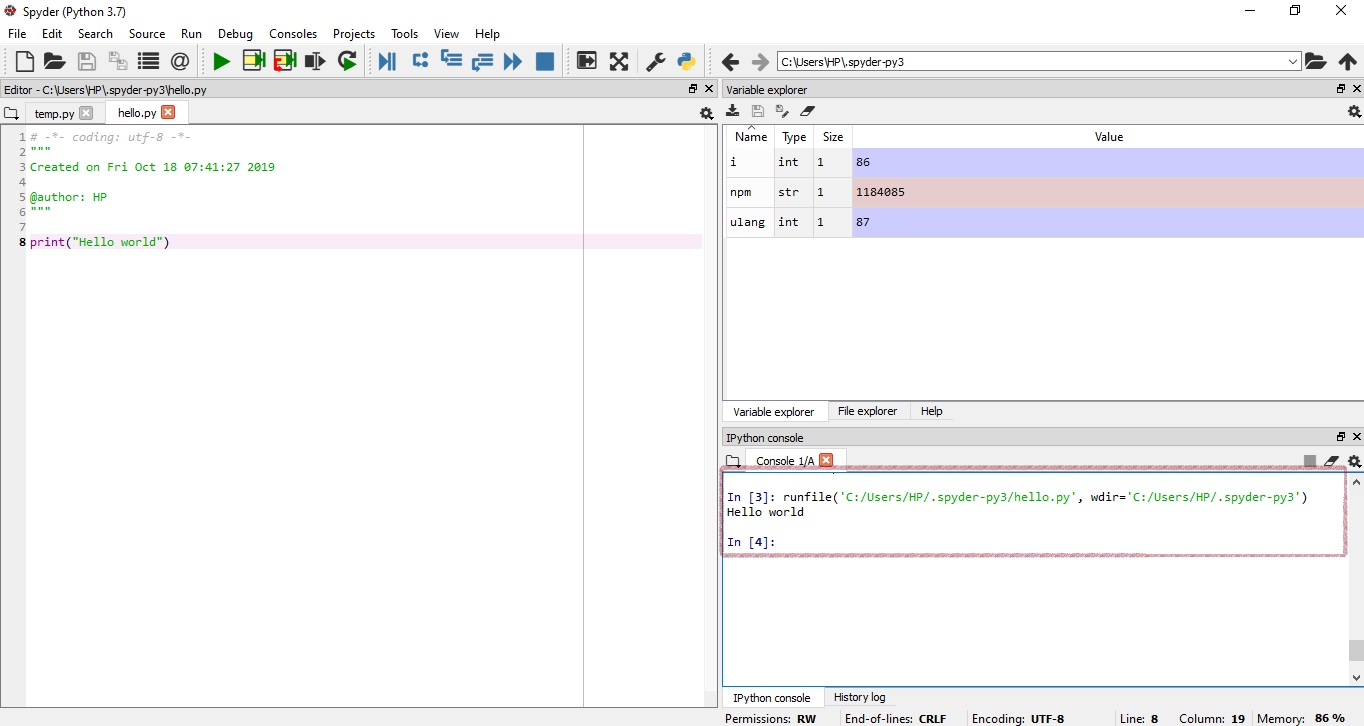
\includegraphics[width=8cm\textwidth]{spyder4.jpg}
    \end{center}
\end{enumerate}
\section{Variable Explorer}
\usepackage{Variable Explore berada di bagian kanan atas berisikan Name, Type, Size. Variable sendiri dapat terisi secara otomatis selama kita menginputkan variable }
\begin{center}
    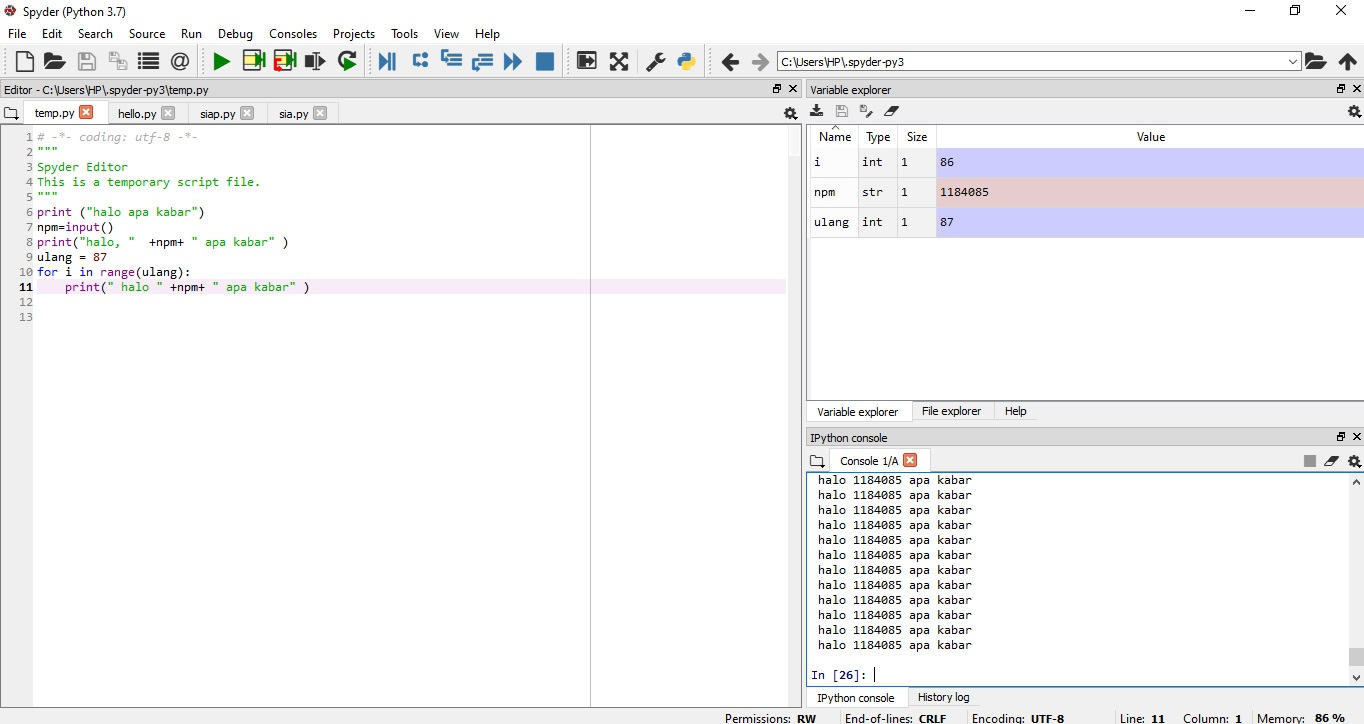
\includegraphics[width=11cm\textwidth]{variable.jpg}
\end{center}

\section{Identasi}
\usepackage{Identasi adalah suatu kesatuan Kode program yang berada pada sisi kiri maka dibaca sebagai satu blok, untuk membuat sub blok maka cukup dengan memberikan jarak spasi atau tab ke kanan. Biasanya dalam Python identasi terjadi saat pencabangan, perulangan, fungsi, class, dan if bersarang.}
\begin{center}
    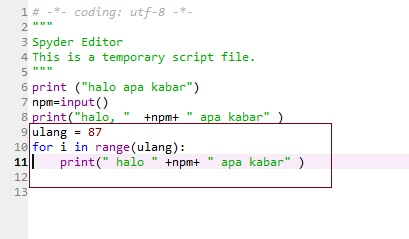
\includegraphics[width=11cm\textwidth]{identasi.jpg}
\end{center}
\end{document}

